% ============================================================
%  Monografía: Cálculo Estocástico
% ============================================================
\documentclass[12pt, a4paper]{report}

% ---- Codificación y lenguaje ----
\usepackage[utf8]{inputenc}
\usepackage[T1]{fontenc}
\usepackage[spanish]{babel}

% ---- Tipografía ----
\usepackage{lmodern}
\usepackage{microtype}

% ---- Matemáticas ----
\usepackage{amsmath, amssymb, amsthm}
\usepackage{mathtools}
\usepackage{dsfont}

% ---- Gráficos ----
\usepackage{graphicx}
\usepackage{float}
\usepackage{tikz}
\usepackage{pgfplots}
\pgfplotsset{compat=1.14}

% ---- Tablas ----
\usepackage{booktabs}
\usepackage{array}

% ---- Notas y TODOs ----
\usepackage[colorinlistoftodos, textsize=small]{todonotes}

% ---- Hipervínculos y referencias ----
\usepackage[colorlinks=true, linkcolor=blue!60!black,
            citecolor=green!50!black, urlcolor=blue]{hyperref}
\usepackage[capitalise, spanish]{cleveref}

% ---- Bibliografía ----
\usepackage[backend=biber, style=alphabetic, sorting=nyt]{biblatex}
\addbibresource{references.bib}

% ---- Diseño de página ----
\usepackage[top=2cm, bottom=2.5cm, left=2.5cm, right=2.5cm]{geometry}
\usepackage{fancyhdr}
\setlength{\headheight}{15pt}
\pagestyle{fancy}
\fancyhf{}
\fancyhead[R]{\thepage}
\fancyhead[L]{\nouppercase{\leftmark}}
\renewcommand{\headrulewidth}{0.4pt}

% ---- Títulos de capítulo (sin salto de página, espacio mínimo) ----
\usepackage{etoolbox}
\makeatletter
\patchcmd{\chapter}{\if@openright\cleardoublepage\else\clearpage\fi}{\par\bigskip}{}{}
\def\@makechapterhead#1{%
  \vspace*{4\p@}%
  {\parindent \z@ \raggedright \normalfont
    \ifnum \c@secnumdepth >\m@ne
      \Large\bfseries \thechapter.\enskip
    \fi
    \interlinepenalty\@M
    \Large\bfseries #1\par\nobreak
    \vskip 10\p@
  }}
\def\@makeschapterhead#1{%
  \vspace*{4\p@}%
  {\parindent \z@ \raggedright \normalfont
    \interlinepenalty\@M
    \Large\bfseries #1\par\nobreak
    \vskip 10\p@
  }}
\makeatother

% ---- Ruta de imágenes ----
\graphicspath{{./}{../}}

% ---- Entornos matemáticos ----
\theoremstyle{plain}
\newtheorem{theorem}{Teorema}[chapter]
\newtheorem{lemma}[theorem]{Lema}
\newtheorem{proposition}[theorem]{Proposición}
\newtheorem{corollary}[theorem]{Corolario}

\theoremstyle{definition}
\newtheorem{definition}[theorem]{Definición}
\newtheorem{example}{Ejemplo}[chapter]

\theoremstyle{remark}
\newtheorem{remark}[theorem]{Observación}
\newtheorem{notation}[theorem]{Notación}

% ---- Macros frecuentes ----
\newcommand{\R}{\mathbb{R}}
\newcommand{\E}{\mathbb{E}}
\newcommand{\Prob}{\mathbb{P}}
\newcommand{\F}{\mathcal{F}}
\newcommand{\N}{\mathbb{N}}
\newcommand{\dd}{\,\mathrm{d}}
\newcommand{\abs}[1]{\left|#1\right|}
\newcommand{\norm}[1]{\left\|#1\right\|}
\newcommand{\inner}[2]{\left\langle#1,\,#2\right\rangle}

% ============================================================
\begin{document}

% ---- Portada ----
\begin{titlepage}
  \centering
  \vspace*{2cm}
  {\Large Universidad de Buenos Aires \par}
  \vspace{0.5cm}
  {\large Facultad de Ciencias Exactas y Naturales \par}
  {\large Cálculo Estocástico \par}
  \vspace{3cm}
  {\Huge\bfseries Difusiones y Score \par}
  \vspace{0.3cm}
  {\Large\bfseries La matemática detrás de los modelos generativos modernos \par}  
  \vspace{2cm}
  {\large Autor: Gonzalo Josué Spina \par}
  \vspace{0.5cm}  
  \vfill
  {\large Julio de 2026 \par}
\end{titlepage}

\clearpage

% ---- Índice ----
\tableofcontents

\clearpage

% ---- Capítulos ----

\chapter{Introducción}
\label{chap:introduccion}

Los modelos de difusión se volvieron muy populares en el último tiempo, al punto tal que estamos comenzando a ver cortos y videos en redes sociales y plataformas de streaming que se asemejan a producciones hollywoodenses con presupuestos millonarios. Esta monografía pretende presentar, en forma ordenada y resumida, los principales resultados que sustentan y dan lugar a las ecuaciones que explican el principio de funcionamiento de estos modelos.

Podemos pensar en los datos (ya sean imágenes, audio o incluso texto que encontramos en diferentes fuentes o generamos a través de una cámara) como realizaciones de una distribución subyacente desconocida, de la cual, si logramos obtener una buena estimación, podemos generar un sinfín de muestras distintas.

El método consiste en partir de un dataset o conjunto de realizaciones, siendo estas representativas de la distribución subyacente y cuya función de distribución poblacional desconocemos; agregar ruido progresivamente en el tiempo mediante una ecuación diferencial estocástica; obtener una nueva distribución en un tiempo final $T$; y luego realizar el camino inverso para obtener una estimación de la distribución original. Este proceso de agregado de ruido, como veremos, no es ad hoc, y la posterior estimación de la distribución original depende de poder estimar con precisión la evolución de su función de densidad a lo largo del tiempo para construir la dinámica inversa.

\chapter{Procesos de Difusión}
\label{chap:difusion}

Dentro del marco teórico de las ecuaciones diferenciales estocásticas, definimos una difusión como un proceso estocástico $X_t = X(t,\omega)$ que satisface una ecuación diferencial estocástica de Itô (EDE) de la forma
\begin{equation}
  \dd X_t = u(t,X_t)\,\dd t + \sigma(t,X_t)\,\dd B_t,
  \label{eq:sde}
\end{equation}
con condición inicial $X_0 = Z$, donde
\[
  u : [0,T] \times \R^d \longrightarrow \R^d
\]
es una función que determina la evolución determinista del proceso,
\[
  \sigma : [0,T] \times \R^d \longrightarrow \R^{d \times m}
\]
determina la intensidad y la dirección del ruido, y $B_t$ es un movimiento browniano $m$-dimensional respecto de una filtración $(\F_t)_{t \geq 0}$. La solución $X_t$ debe ser, a su vez, un proceso adaptado a esta filtración.

Equivalentemente,~\eqref{eq:sde} se interpreta en su forma integral como
\begin{equation}
  X_t = Z + \int_0^t u(s,X_s)\,\dd s + \int_0^t \sigma(s,X_s)\,\dd B_s.
  \label{eq:sde-integral}
\end{equation}

El coeficiente $u(t,x)$ se conoce como \emph{drift} o coeficiente de deriva, mientras que $\sigma(t,x)$ se denomina coeficiente de difusión. El primero describe la evolución local determinista del proceso, mientras que el segundo determina cómo actúa el ruido browniano sobre este.

El siguiente teorema muestra que, si imponemos ciertas condiciones sobre ambos coeficientes, la ecuación posee una única solución. Aunque esta solución no siempre puede calcularse de forma explícita, es posible aproximarla mediante métodos numéricos.

\begin{theorem}[Existencia y unicidad]
\label{thm:existencia-unicidad}
Sean $u$ y $\sigma$ funciones medibles para las cuales existen constantes $C, D > 0$ tales que, para todo $t \in [0,T]$ y $x, y \in \R^d$,
\begin{equation}
  \norm{u(t,x) - u(t,y)} + \norm{\sigma(t,x) - \sigma(t,y)} \leq C\norm{x - y},
  \label{eq:lipschitz}
\end{equation}
y
\begin{equation}
  \norm{u(t,x)}^2 + \norm{\sigma(t,x)}^2 \leq D\bigl(1 + \norm{x}^2\bigr).
  \label{eq:crecimiento}
\end{equation}
Si $Z$ es $\F_0$-medible y satisface $\E[\norm{Z}^2] < \infty$, entonces la EDE
\[
  \dd X_t = u(t,X_t)\,\dd t + \sigma(t,X_t)\,\dd B_t, \qquad X_0 = Z,
\]
admite una única solución fuerte y continua $X_t$ en el intervalo $[0,T]$.
\end{theorem}

La condición~\eqref{eq:lipschitz} es una condición de Lipschitz global y garantiza la unicidad de la solución, mientras que la condición~\eqref{eq:crecimiento}, denominada condición de crecimiento lineal, evita que la solución explote en tiempo finito.

\begin{notation}
\label{not:ex}
Escribimos $\E^x[\,\cdot\,] := \E[\,\cdot \mid X_0 = x]$ para denotar la esperanza condicionada al evento $\{X_0 = x\}$.
\end{notation}

\begin{example}[Proceso de Ornstein--Uhlenbeck]
\label{ex:ou}
El \emph{proceso de Ornstein--Uhlenbeck} (OU) es la difusión en $\R$ definida por
\begin{equation}
  \dd X_t = -X_t\,\dd t + \sigma\,\dd B_t, \qquad X_0 = x_0,
  \label{eq:ou}
\end{equation}
con $\sigma > 0$. Los coeficientes $u(t,x) = -x$ y $\sigma(t,x) = \sigma$ son globalmente Lipschitz y de crecimiento lineal, de modo que el Teorema~\ref{thm:existencia-unicidad} garantiza existencia y unicidad de la solución.

La solución explícita se obtiene por variación de la constante:
\[
  X_t = x_0\,e^{-t} + \sigma\int_0^t e^{-(t-s)}\,\dd B_s.
\]
Por las propiedades de la integral de Itô, $X_t \mid X_0 = x_0$ es gaussiana con
\[
  \E^{x_0}[X_t] = x_0\,e^{-t},
  \qquad
  \mathrm{Var}(X_t \mid X_0 = x_0) = \frac{\sigma^2}{2}\bigl(1 - e^{-2t}\bigr).
\]
Cuando $t \to \infty$, la media tiende a $0$ y la varianza tiende a $\sigma^2/2$, independientemente del valor inicial $x_0$: la distribución de $X_t$ converge a $\mathcal{N}(0,\,\sigma^2/2)$.

\begin{figure}[H]
  \centering
  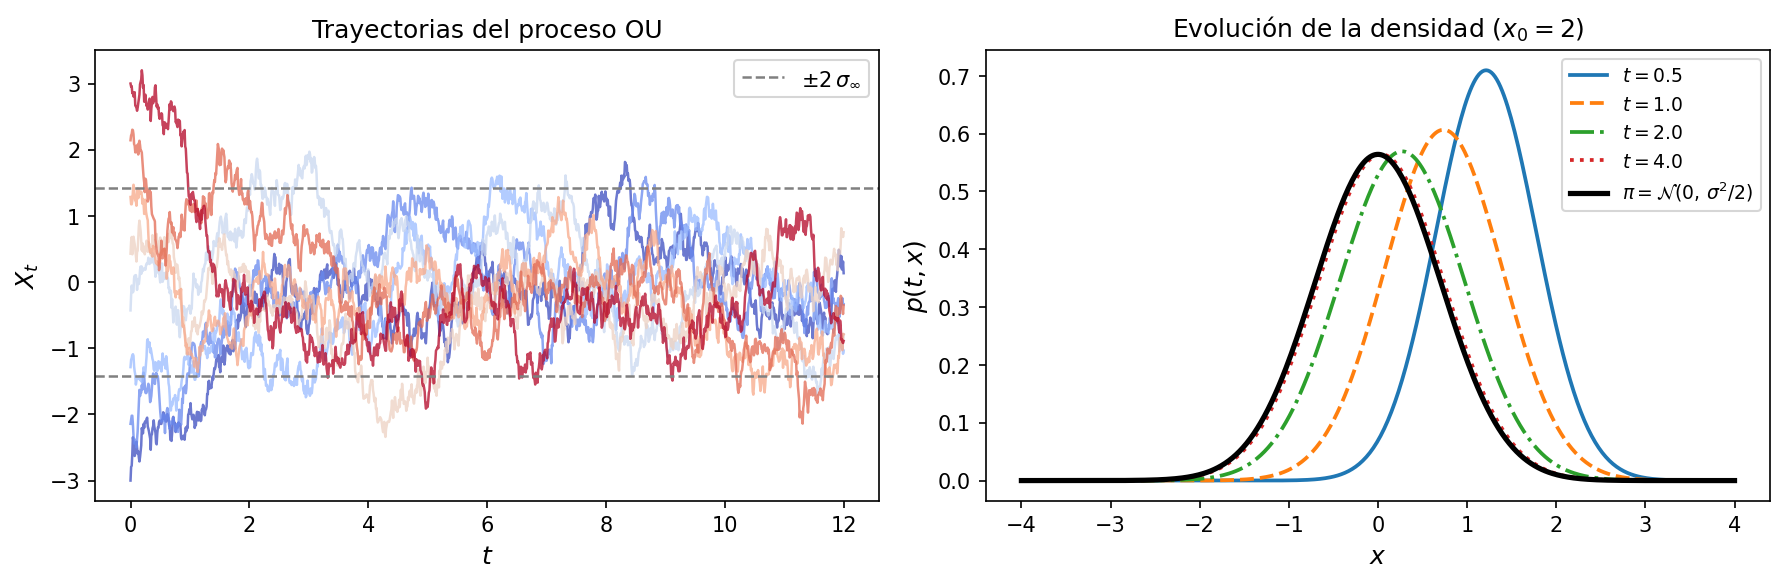
\includegraphics[width=\textwidth]{ou_trajectories.png}
  \caption{Izquierda: trayectorias del proceso OU con $\sigma = 1$ partiendo de distintas condiciones iniciales $x_0 \in [-3,3]$. Las líneas punteadas indican la banda $\pm 2\sigma_\infty$ de la distribución estacionaria. Derecha: densidad $p(t,\cdot)$ partiendo de $x_0 = 2$ en distintos instantes; la curva negra es $\pi = \mathcal{N}(0,\sigma^2/2)$.}
  \label{fig:ou-trayectorias}
\end{figure}
\end{example}

\chapter{Evolución de la densidad de un proceso}
\label{chap:generador}

El objetivo de este capítulo es entender cómo evoluciona en el tiempo la distribución de un proceso de difusión. Dado que la densidad $p_t(x) = p(t,x)$ del proceso $X_t$ contiene toda la información de su distribución en el instante $t$, conocerla nos permite entender y reconstruir dicha distribución por completo. Más precisamente, si $X_t$ admite una densidad $p(t,x)$, queremos caracterizar la ecuación en derivadas parciales que esta densidad satisface. Para llegar a ese resultado necesitamos introducir antes el generador infinitesimal del proceso, que describe la tasa de cambio de la esperanza de cualquier observable, y las ecuaciones de Kolmogorov, que conectan esa perspectiva con la evolución de $p(t,x)$.

Como las difusiones son procesos de Markov, la cantidad $\E^x[f(X_{t+h})]$ depende únicamente del estado actual $x$, no de toda la historia del proceso. Esto permite definir el siguiente operador, que cuantifica la tasa de cambio de la esperanza de cualquier observable $f : \R^d \to \R$ en función del punto de partida.

\begin{definition}[Generador infinitesimal]
\label{def:generador}
Sea $(X_t)_{t \geq 0}$ una difusión de Markov. Su \emph{generador infinitesimal} es el operador diferencial lineal definido por
\[
  \mathcal{A}_{t}f(x) = \lim_{h \downarrow 0} \frac{\E^x[f(X_{t+h})] - f(x)}{h},
\]
para toda función $f \in \mathcal{D}_{\mathcal{A}}(x)$, donde $\mathcal{D}_{\mathcal{A}}(x)$ es el conjunto de funciones para las cuales este límite existe en $x$.
\end{definition}

El generador puede interpretarse como el análogo de la derivada en el cálculo diferencial: describe la tasa instantánea de variación de la esperanza del observable $f(X_t)$.

Los siguientes resultados nos permiten calcular el generador de un proceso.

\begin{lemma}
\label{lem:ito-esperanza}
Sea $X_t$ un proceso en $\R^d$ de la forma
\[
  X_t(\omega) = x + \int_0^t u(s,\omega)\,\dd s + \int_0^t v(s,\omega)\,\dd B_s(\omega),
\]
con $X_0 = x$. Sea $f \in C^2(\R^d)$ con soporte compacto. Supongamos que $u(t,\omega)$ y $v(t,\omega)$ son acotadas en $(t,\omega)$ de forma tal que $X_t(\omega)$ permanece en el soporte de $f$. Entonces
\[
  \E^x[f(X_t)]
  = f(x)
  + \E^x\!\left[\int_0^t \left(
      \sum_{i=1}^{d} u_i(s,\omega)\,\frac{\partial f}{\partial x_i}(X_s)
      + \frac{1}{2}\sum_{i,j=1}^{d} (vv^{\top})_{i,j}(s,\omega)\,
        \frac{\partial^2 f}{\partial x_i\,\partial x_j}(X_s)
    \right)\dd s\right].
\]
\end{lemma}

\begin{theorem}
\label{thm:generador-difusion}
Sea $X_t$ una difusión que satisface la ecuación~\eqref{eq:sde} y sea $f \in C_0^2(\R^d)$. Entonces $f \in \mathcal{D}(\mathcal{A})$ y
\begin{equation}
  \label{eq:generador}
  \mathcal{A}_t f(x) = \sum_{i=1}^{d} u_i(t,x)\,\frac{\partial f}{\partial x_i}(x)
  + \frac{1}{2}\sum_{i,j=1}^{d} (\sigma\sigma^{\top})_{i,j}(t, x)\,
  \frac{\partial^2 f}{\partial x_i\,\partial x_j}(x).
\end{equation}
\end{theorem}

Combinando el Lema~\ref{lem:ito-esperanza} y el Teorema~\ref{thm:generador-difusion}, obtenemos el equivalente al teorema central del cálculo.

\begin{theorem}[Fórmula de Dynkin]
\label{thm:dynkin}
Sea $f \in C^2(\R^d)$. Entonces
\begin{equation}
  \label{eq:dynkin}
  \E^x[f(X_t)]
  = f(x) + \E^x\!\left[\int_0^t \mathcal{A}_s f(X_s)\,\dd s\right].
\end{equation}
\end{theorem}

La fórmula de Dynkin, además de ser un resultado central en sí mismo, es el ingrediente clave para obtener las dos ecuaciones de Kolmogorov. La primera, que presentamos a continuación, describe cómo evoluciona la esperanza de un observable condicionada al estado actual; la segunda, que derivaremos enseguida, gobierna la evolución de la densidad.

\begin{theorem}[Ecuación de Kolmogorov hacia atrás]
\label{thm:kolmogorov-backward}
Sea $X_t$ una difusión que satisface~\eqref{eq:sde}, sea $T > 0$ y sea $f \in C^2_b(\R^d)$. Supongamos además que los coeficientes $u^i$ y $a^{ij} = (\sigma\sigma^\top)^{ij}$ son Hölder continuos en $(t,x)$ y que $a$ es uniformemente elíptica, es decir, existe $\lambda > 0$ tal que
\[
  \sum_{i,j=1}^d a^{ij}(t,x)\,\xi_i\xi_j \geq \lambda|\xi|^2
  \qquad \forall\,(t,x) \in [0,T]\times\R^d,\;\forall\,\xi \in \R^d.
\]
Entonces la función $v(t,x) = \E^x\bigl[f(X_T)\bigr]$ pertenece a $C^{1,2}([0,T)\times\R^d)$ y es la única solución clásica de
\[
  \frac{\partial v}{\partial t}(t,x) + \mathcal{A}_t v(t,x) = 0,
  \qquad (t,x) \in [0,T) \times \R^d,
\]
con condición terminal $v(T,x) = f(x)$.
\end{theorem}

Para encontrar la ecuación que gobierna la densidad $p(t,x)$, partimos de la fórmula de Dynkin. Supongamos que $X_t$ admite una densidad $p(t,\cdot)$ para cada $t \geq 0$. Reescribiendo la esperanza como integral contra $p$:
\[
  \int_{\R^d} f(x)\,p(t,x)\,\dd x
  = \int_{\R^d} f(x)\,p(0,x)\,\dd x
  + \int_0^t \int_{\R^d} \mathcal{A}_s f(x)\,p(s,x)\,\dd x\,\dd s.
\]
Diferenciando respecto de $t$ (el intercambio con la integral se justifica por convergencia dominada bajo la hipótesis $p \in C^{1,2}(\R^d)$):
\[
  \frac{\dd}{\dd t}\int_{\R^d} f(x)\,p(t,x)\,\dd x
  = \int_{\R^d} f(x)\,\frac{\partial p}{\partial t}(t,x)\,\dd x
  = \int_{\R^d} \mathcal{A}_t f(x)\,p(t,x)\,\dd x.
\]
Queremos trasladar el operador $\mathcal{A}_t$ de $f$ a $p$. Para ello definimos su adjunto en $L^2(\R^d)$.

\begin{definition}[Operador adjunto del generador]
\label{def:adjunto}
El \emph{operador adjunto} $\mathcal{A}_t^*$ es el operador que satisface
\[
  \int_{\R^d} (\mathcal{A}_t f)(x)\,p(x)\,\dd x
  = \int_{\R^d} f(x)\,(\mathcal{A}_t^* p)(x)\,\dd x
\]
para toda $f \in C_0^2(\R^d)$ y toda densidad $p$ suficientemente regular.
\end{definition}

Con esta definición la ecuación anterior se reescribe como
\[
  \int_{\R^d} f(x)\,\frac{\partial p}{\partial t}(t,x)\,\dd x
  = \int_{\R^d} f(x)\,\bigl(\mathcal{A}_t^*\, p(t,\cdot)\bigr)(x)\,\dd x,
\]
y como esto vale para toda $f \in C_0^2(\R^d)$, concluimos que $p$ satisface la siguiente ecuación.

\begin{theorem}[Fokker-Planck]
\label{thm:fokker-planck}
Bajo las mismas hipótesis de regularidad y elipticidad del Teorema~\ref{thm:kolmogorov-backward}, sea $p_0 \in C(\R^d) \cap L^1(\R^d)$ una densidad de probabilidad. Entonces existe una única densidad $p \in C^{1,2}((0,T]\times\R^d)$ que satisface
\[
  \frac{\partial p}{\partial t} = \mathcal{A}_t^*\, p,
\]
con condición inicial $p(0,x) = p_0(x)$. Calculando explícitamente $\mathcal{A}_t^*$ mediante integración por partes a partir del Teorema~\ref{thm:generador-difusion}:
\begin{equation}
  \label{eq:fokker-planck}
  \frac{\partial p}{\partial t}
  = -\sum_{i=1}^{d} \frac{\partial}{\partial x_i}\bigl[u_i(t,x)\,p(t,x)\bigr]
  + \frac{1}{2}\sum_{i,j=1}^{d}
    \frac{\partial^2}{\partial x_i\,\partial x_j}
    \bigl[(\sigma\sigma^{\top})_{i,j}(t,x)\,p(t,x)\bigr].
\end{equation}
\end{theorem}

\begin{example}[Fokker-Planck del proceso OU]
\label{ex:fp-ou}
Para el proceso OU~\eqref{eq:ou} con $u(t,x) = -x$ y $a(t,x) = \sigma^2$, la ecuación de Fokker-Planck toma la forma
\[
  \frac{\partial p}{\partial t} = \frac{\partial}{\partial x}(x\,p)
  + \frac{\sigma^2}{2}\frac{\partial^2 p}{\partial x^2}.
\]
Se verifica directamente que la densidad de $\mathcal{N}(0,\,\sigma^2/2)$ satisface $\mathcal{A}^*p_\infty = 0$: es la distribución estacionaria del proceso, en acuerdo con la solución explícita del Ejemplo~\ref{ex:ou}.
\end{example}

\chapter{Reverse Time Diffusion}
\label{chap:reverse}

Hasta aquí hemos estudiado cómo un proceso de difusión que parte de una distribución inicial $X_0$ evoluciona hacia adelante en el tiempo. En este capítulo nos interesa el camino inverso: dado un proceso en el instante $T > 0$, construir un proceso que corra hacia atrás y recupere la distribución original de $X_0$. Veremos que este proceso inverso es también una difusión.

Para formalizar la idea, definimos el proceso con el tiempo invertido como
\[
  \hat{X}_t = X_{T-t}, \qquad t \in [0,T],
\]
y buscamos coeficientes $\hat{u}$, $\hat{\sigma}$ y un movimiento browniano $\hat{B}_t$ tales que $\hat{X}_t$ satisfaga una EDE. Puede demostrarse que el proceso invertido conserva la propiedad de Markov (usando la inversión temporal de la propiedad de Markov de $X_t$). El contenido no trivial del resultado es que $\hat{X}_t$ satisface una EDE, lo que requiere construir explícitamente un proceso auxiliar $\tilde{B}_t$ y demostrar que posee la propiedad de movimiento browniano respecto de la filtración \emph{decreciente} $\mathcal{F}^\downarrow_t = \sigma(X_s, \tilde{B}_s : s \geq t)$. Esto es lo que demuestra Anderson \cite{Anderson1982} en su Sección~4.

\begin{theorem}[Inversión temporal, Anderson]
\label{thm:time-reversal}
Supongamos que $u$ y $\sigma$ satisfacen las condiciones del Teorema~\ref{thm:existencia-unicidad}, y que $X_t$ admite una densidad $p(t,x)$ que satisface la ecuación de Fokker-Planck (Teorema~\ref{thm:fokker-planck}), con $p \in C^{1,2}([0,T]\times\R^d)$ y $p(t,x) > 0$ para todo $(t,x)$.
Denotamos $a(t,x) = \sigma(t,x)\sigma(t,x)^{\top}$ y definimos
\begin{align*}
  \hat{u}^{\,i}(t,x) &= -u^i(T-t,x)
    + \frac{1}{p(T-t,x)}\frac{\partial}{\partial x_j}
      \bigl[a^{ij}(T-t,x)\,p(T-t,x)\bigr], \\
  \hat{\sigma}(t,x) &= \sigma(T-t,x),
\end{align*}
con la convención de que $\hat{u}^{\,i}(t,x) = 0$ cuando $p(T-t,x) = 0$. Entonces existe un movimiento browniano $r$-dimensional $\hat{B}_t$ tal que $(\hat{X}_t)_{0 \leq t \leq T}$ es una difusión de Markov que satisface
\[
  \dd\hat{X}_t = \hat{u}(t,\hat{X}_t)\,\dd t + \hat{\sigma}(t,\hat{X}_t)\,\dd\hat{B}_t,
\]
con generador
\[
  \hat{\mathcal{A}}_t f(x)
  = \frac{1}{2}\sum_{i,j=1}^{d} a^{ij}(T-t,x)\,\frac{\partial^2 f}{\partial x_i\,\partial x_j}(x)
  + \sum_{i=1}^{d} \hat{u}^{\,i}(t,x)\,\frac{\partial f}{\partial x_i}(x).
\]
\end{theorem}

\begin{proof}
\noindent\textbf{Paso 1: identificación del generador.}
Sea $f \in C_0^2(\R^d)$ y denotemos $p_t = p(t,\cdot)$. Por definición del generador:
\[
  \hat{\mathcal{A}}_t f(x)
  = \lim_{h\downarrow 0}\frac{\E[f(X_{T-t-h})\mid X_{T-t}=x]-f(x)}{h}.
\]
Escribimos $p_{X_r \mid X_s=y}(x)$ para la densidad de transición del proceso forward: la densidad de $X_r$ dado $X_s = y$, evaluada en $x$, con $s < r$. Denotamos $g(h) = \E[f(X_{T-t-h})\mid X_{T-t}=x]$. Aplicando la fórmula de Bayes para densidades condicionales para pasar de la transición forward $p_{X_{T-t} \mid X_{T-t-h}=y}(x)$ a la condicional backward $p_{X_{T-t-h} \mid X_{T-t}=x}(y)$:
\[
  g(h)
  = \int_{\R^d} f(y)\,\frac{p_{X_{T-t} \mid X_{T-t-h}=y}(x)\;p_{T-t-h}(y)}{p_{T-t}(x)}\,\dd y.
\]
Para $h > 0$, la densidad de transición $p_{X_{T-t} \mid X_{T-t-h}=y}(x)$ es suave en $y$ por regularidad elíptica. Aplicando la regla del producto al integrando:

\smallskip
\emph{Término (I).} La ecuación de Kolmogorov backward establece, para $h > 0$:
\[
  \frac{d}{dh}\,p_{X_{T-t} \mid X_{T-t-h}=y}(x) = \mathcal{A}_{T-t-h}^y\,p_{X_{T-t} \mid X_{T-t-h}=y}(x).
\]

\emph{Término (II).} Por la ecuación de Fokker-Planck:
\[
  \frac{d}{dh}\,p_{T-t-h}(y) = -(\mathcal{A}_{T-t-h}^*\,p_{T-t-h})(y).
\]

Como $p_{X_{T-t} \mid X_{T-t-h}=y}(x)$ es suave para $h > 0$, la dualidad en $L^2$ se aplica sin restricciones al Término (I). Combinando ambos términos:
\[
  p_{T-t}(x)\,\frac{d}{dh}\,g(h)
  = \int_{\R^d} p_{X_{T-t} \mid X_{T-t-h}=y}(x)
    \bigl[(\mathcal{A}_{T-t-h}^*(f\cdot p_{T-t-h}))(y)
    - f(y)\,(\mathcal{A}_{T-t-h}^*\,p_{T-t-h})(y)\bigr]\,\dd y.
\]
Reescribiendo el factor $p_{X_{T-t} \mid X_{T-t-h}=y}(x)\,p_{T-t-h}(y) = p_{T-t}(x)\,p_{X_{T-t-h} \mid X_{T-t}=x}(y)$ mediante Bayes y expandiendo con la regla de Leibniz sobre $\mathcal{A}^*$:
\[
  \frac{d}{dh}\,g(h)
  = \int_{\R^d} p_{X_{T-t-h} \mid X_{T-t}=x}(y)
    \left[\frac{1}{2}\sum_{i,j}a^{ij}_{T-t-h}(y)\,\partial_{y_iy_j}^2f
    + \sum_i c^i_h(y)\,\partial_{y_i}f\right]\dd y,
\]
donde $c^i_h(y) = -u^i_{T-t-h}(y) + \tfrac{\partial_{y_j}(a^{ij}_{T-t-h}(y)\,p_{T-t-h}(y))}{p_{T-t-h}(y)}$.
Tomando $h \to 0^+$: la distribución condicional $p_{X_{T-t-h} \mid X_{T-t}=x}$ converge débilmente a la masa puntual en $x$, de modo que la integral evalúa el integrando en $y = x$ y $h = 0$:
\[
  \hat{\mathcal{A}}_t f(x)
  = \frac{1}{2}\sum_{i,j}a^{ij}(T{-}t,x)\,\frac{\partial^2 f}{\partial x_i\partial x_j}
  + \sum_i \hat{u}^{\,i}(t,x)\,\frac{\partial f}{\partial x_i},
\]
con $\hat{u}^i(t,x) = -u^i(T{-}t,x) + \tfrac{\partial_{x_j}(a^{ij}(T{-}t,x)\,p_{T-t}(x))}{p_{T-t}(x)}$, que coincide exactamente con los coeficientes del enunciado.

\medskip
\noindent\textbf{Paso 2: construcción de $\hat{B}_t$ (Anderson \cite{Anderson1982}, Secc.\,4).}

Trabajamos en tiempo forward $t \in [t_0, T]$. Definimos el proceso auxiliar $\tilde{B}_t$ ($r$-dimensional) por $\tilde{B}_{t_0} = 0$ y
\[
  \dd\tilde{B}_t^k = \dd B_t^k
  + \frac{1}{p(t,X_t)}\sum_{j=1}^d
    \frac{\partial}{\partial x^j}\bigl[p(t,X_t)\,\sigma^{jk}(t,X_t)\bigr]\,\dd t,
  \quad k=1,\ldots,r.
\]
El proceso conjunto $(X_t,\tilde{B}_t)$ satisface el sistema:
\begin{align}
  \dd X_t^i &= u^i(t,X_t)\,\dd t + \sum_k \sigma^{ik}(t,X_t)\,\dd B_t^k, \tag{A}\label{eq:A}\\[2pt]
  \dd\tilde{B}_t^k &= \dd B_t^k
    + \frac{1}{p(t,X_t)}\sum_j\frac{\partial(p\,\sigma^{jk})}{\partial x^j}(t,X_t)\,\dd t.
    \tag{B}\label{eq:B}
\end{align}

\smallskip
\noindent\textbf{Lema 1.}
\textit{Sea $\phi(\beta,t) = [2\pi(t-t_0)]^{-r/2}\exp\!\bigl(-\|\beta\|^2/[2(t-t_0)]\bigr)$. La densidad conjunta de $(X_t,\tilde{B}_t)$ factoriza como $p(x,\beta,t) = p(x,t)\,\phi(\beta,t)$.}
\begin{proof}
La ecuación de Fokker-Planck para la densidad conjunta de \eqref{eq:A}--\eqref{eq:B} tiene términos de deriva y difusión en $x$, en $\tilde{B}$ y cruzados $(x,\tilde{B})$. Sustituimos el ansatz $p(x,t)\phi(\beta,t)$: los términos en $x$ dan $\phi\,\partial_t p$; los de difusión en $\tilde{B}$ dan $p\,\partial_t\phi$ por la ecuación del calor. Los términos de deriva en $\tilde{B}$ y de difusión cruzada tienen la forma $\pm(\partial_{\beta^k}\phi)\cdot\sum_j\partial_{x^j}(p\sigma^{jk})$ y se cancelan entre sí. Queda $\partial_t(p\phi)$, que coincide con el lado izquierdo. La condición inicial $p(x,\beta,t_0)=p(x,t_0)\delta(\beta)$ se verifica, y la unicidad da la factorización.
\end{proof}

\smallskip
\noindent\textbf{Lema 2.}
\textit{$X_t$ y $\tilde{B}_t-\tilde{B}_s$ son independientes para todo $t\geq s\geq t_0$.}
\begin{proof}
Del Lema 1, $p(\tilde{B}_t\mid X_t=x,t)=\phi(\tilde{B}_t,t)$ no depende de $x$, luego $X_t$ y $\tilde{B}_t$ son independientes. Repitiendo el argumento condicionando en $\tilde{B}_s$ se obtiene que $\tilde{B}_t-\tilde{B}_s\sim\mathcal{N}(0,(t-s)I)$ independientemente de $X_t$ (Anderson, Lemas 3--5).
\end{proof}

\smallskip
\noindent\emph{$\tilde{B}_t$ como browniano hacia atrás.}
Definimos la filtración \emph{decreciente} $\mathcal{F}^\downarrow_t := \sigma(X_s,\tilde{B}_s:s\geq t)$. Del Lema~2, $\tilde{B}_t-\tilde{B}_{t+s}$ es independiente de $\mathcal{F}^\downarrow_{t+s}$ y tiene distribución $\mathcal{N}(0,sI)$, lo que da las condiciones de movimiento browniano respecto de $\mathcal{F}^\downarrow_t$:
\begin{align*}
  \E\bigl[\tilde{B}_t \mid \mathcal{F}^\downarrow_{t+s}\bigr] &= \tilde{B}_{t+s}, \\
  \E\bigl[(\tilde{B}_t-\tilde{B}_{t+s})(\tilde{B}_t-\tilde{B}_{t+s})^\top \mid \mathcal{F}^\downarrow_{t+s}\bigr]
    &= s\,I.
\end{align*}

\smallskip
\noindent\emph{EDE del proceso inverso.}
Despejando $\dd B_t^k$ de \eqref{eq:B} y sustituyendo en \eqref{eq:A}:
\[
  \dd X_t^i
  = \Bigl[u^i - \tfrac{1}{p}\sum_j\partial_{x^j}(p\,a^{ij})\Bigr]\dd t
  + \sum_k\sigma^{ik}\,\dd\tilde{B}_t^k,
\]
usando $\sum_k\sigma^{ik}\sigma^{jk}=a^{ij}$ y la corrección de Stratonovich para integrales hacia atrás (Anderson \cite{Anderson1982}, p.\,321). Reparametrizando con $\tau=T-t$, $\hat{X}_\tau=X_{T-\tau}$ y
\[
  \hat{B}_\tau = \tilde{B}_T - \tilde{B}_{T-\tau},
\]
que es un movimiento browniano estándar respecto de la filtración natural de $\hat{X}$, se obtiene la EDE del enunciado:
\[
  \dd\hat{X}_\tau = \hat{u}(\tau,\hat{X}_\tau)\,\dd\tau
  + \sigma(T-\tau,\hat{X}_\tau)\,\dd\hat{B}_\tau. \qedhere
\]
\end{proof}

\chapter{Score y Song}
\label{chap:score}

En su paper de 2021, Song et al.\ \cite{Song2021} introducen un framework unificado para la generación de datos que descansa enteramente en la maquinaria que desarrollamos en los capítulos anteriores. La idea central es la siguiente: dado un conjunto de realizaciones de una distribución desconocida $p_0$, se construye una EDE hacia adelante que transforma progresivamente $p_0$ en una distribución conocida $p_T$ (típicamente una gaussiana) elegida como prior. Gracias al Teorema~\ref{thm:time-reversal}, existe un proceso de difusión que recorre el camino inverso: parte de $p_T$ y recupera $p_0$. El coeficiente de deriva del proceso inverso depende del gradiente del logaritmo de la densidad $p_t$, que se conoce como el \emph{score} del proceso. Si se logra aprender el score para todo $t \in [0, T]$, es posible simular el proceso inverso y generar nuevas muestras de $p_0$.

\paragraph{Ergodicidad y convergencia al prior.}

El proceso forward transforma $p_0$ en $p_T$, pero para poder samplear el punto de partida del proceso inverso necesitamos conocer $p_T$. Si el proceso forward es \emph{ergódico}, es decir, olvida la condición inicial y converge a una única distribución estacionaria $\pi$, entonces para $T$ suficientemente grande $p_T \approx \pi$ independientemente de $p_0$, y podemos samplear desde $\pi$ directamente. El proceso OU satisface esta condición (véase el Ejemplo~\ref{ex:fp-ou}) con $\pi = \mathcal{N}(0,\sigma^2/2)$.

\paragraph{El score y su rol en la difusión inversa.}

\begin{definition}[Score]
\label{def:score}
Dado un proceso de difusión $X_t$ con densidad $p(t,x)$, se define el \emph{score} como
\[
  s(t,x) = \nabla_x \log p(t,x).
\]
\end{definition}

Para ver cómo aparece naturalmente en la dinámica inversa, retomamos el Teorema~\ref{thm:time-reversal}. Cuando $\sigma = \sigma(t)$ depende solo del tiempo, la matriz $a^{ij}(t,x) = \sigma(t)^2\delta^{ij}$ es diagonal y sus derivadas espaciales se anulan. El drift inverso se simplifica a
\[
  \hat{u}(t,x) = -u(T-t,x) + \sigma(T-t)^2\,\nabla_x\log p(T-t,x),
\]
y la EDE del proceso inverso queda
\begin{equation}
  \dd\hat{X}_t = \bigl[-u(T-t,\hat{X}_t) + \sigma(T-t)^2\,\nabla_x\log p(T-t,\hat{X}_t)\bigr]\dd t
  + \sigma(T-t)\,\dd\hat{B}_t.
  \label{eq:reverse-score}
\end{equation}
El score es el único ingrediente de esta ecuación que no está disponible directamente: $u$ y $\sigma$ son coeficientes del proceso forward, elegidos por el modelador, pero $\nabla_x \log p(t,x)$ depende de la distribución desconocida $p_0$ a través de la evolución de la densidad.

\begin{example}[Score y difusión inversa en el proceso OU]
\label{ex:score-ou}
Para el proceso OU~\eqref{eq:ou} con $u(t,x) = -x$ y $\sigma$ constante, el drift inverso~\eqref{eq:reverse-score} queda
\[
  \dd\hat{X}_t = \bigl[\hat{X}_t + \sigma^2\,\nabla_x\log p(T-t,\hat{X}_t)\bigr]\dd t + \sigma\,\dd\hat{B}_t,
\]
partiendo de $\hat{X}_0 \sim \mathcal{N}(0,\sigma^2/2)$. El drift cambia de signo respecto del proceso forward ($-x \to +x$): mientras el forward empuja el proceso hacia $0$, el reverse lo aleja, y el score corrige esa dinámica para recuperar la forma de $p_0$.

Escribimos $p_{X_t \mid X_0=x_0}(x)$ para la densidad de transición del proceso: la densidad de $X_t$ dado $X_0 = x_0$, evaluada en $x$. Por la ley de probabilidad total, la densidad marginal satisface
\[
  p(t,x) = \int p_{X_t \mid X_0=x_0}(x)\,p_0(x_0)\,\dd x_0,
\]
que para el OU queda $p(t,x) = \int \mathcal{N}(x;\,x_0 e^{-t},\,\tfrac{\sigma^2}{2}(1-e^{-2t}))\,p_0(x_0)\,\dd x_0$. Esta integral depende de la desconocida $p_0$, por lo que el score marginal $\nabla_x \log p(T-t,x)$ no es computable directamente. En cambio, como $p_{X_t \mid X_0=x_0}(x)$ es gaussiana, el score condicional evaluado en $x$ es analítico:
\[
  \nabla_x \log p_{X_t \mid X_0=x_0}(x) = -\frac{x - x_0\,e^{-t}}{\tfrac{\sigma^2}{2}(1-e^{-2t})}.
\]
La red $s_\theta(t,x_t)$ se entrena para predecir este score condicional sobre pares $(x_0, x_t)$ generados por el proceso forward, y luego se sustituye como aproximación del score marginal en la EDE inversa.
\end{example}

\paragraph{Aprendizaje del score: denoising score matching.}

El puente formal entre el score marginal y el score condicional es la siguiente identidad \cite{Hyvarinen2005}. Diferenciando $p(t,x) = \int p_{X_t \mid X_0=x_0}(x)\,p_0(x_0)\,\dd x_0$ bajo la integral y aplicando Bayes para reescribir $p_{X_t \mid X_0=x_0}(x)\,p_0(x_0)/p(t,x) = p_{X_0 \mid X_t=x}(x_0)$:
\[
  \nabla_x \log p(t,x)
  = \int \nabla_x \log p_{X_t \mid X_0=x_0}(x)\cdot p_{X_0 \mid X_t=x}(x_0)\,\dd x_0.
\]
Fijado $X_t = x$, se promedia el score condicional (función de $x_0$) contra el posterior de la condición inicial dado que el proceso vale $x$ al tiempo $t$. Vincent \cite{Vincent2011} y Song \& Ermon \cite{Song2021} observaron que el minimizador de $\E[\norm{s_\theta - \nabla_x \log p_t}^2]$ coincide con el del objetivo computable
\[
  \tilde{J}(\theta) = \int_0^T \lambda(t)\,\E_{p_0(x_0)\,p(x_t \mid x_0)}\!\left[
    \norm{s_\theta(t,x_t) - \nabla_{x_t}\log p_{X_t \mid X_0=x_0}(x_t)}^2
  \right]\dd t,
\]
donde la esperanza se toma sobre pares $(x_0, x_t)$ con $x_0 \sim p_0$ y $x_t \mid x_0$ simulado por el proceso forward.

\paragraph{Algoritmo de generación.}

Con $s_\theta$ entrenado se sustituye en la EDE inversa~\eqref{eq:reverse-score} y se integra por Euler--Maruyama \cite{Oksendal2003} con paso $\Delta t = T/N$:

\begin{enumerate}
  \item Samplear $x_T \sim \pi = \mathcal{N}(0,\sigma^2/2)$.
  \item Para $k = N, N-1, \ldots, 1$ con $t_k = k\Delta t$: samplear $z_k \sim \mathcal{N}(0,I)$ y actualizar
  \[
    x_{t_{k-1}} = x_{t_k}
    + \bigl[-u(t_k,x_{t_k}) + \sigma(t_k)^2\,s_\theta(t_k,x_{t_k})\bigr]\Delta t
    + \sigma(t_k)\sqrt{\Delta t}\;z_k.
  \]
  \item Retornar $x_0 \sim p_0$ (aproximado).
\end{enumerate}

\paragraph{Experimento numérico.}

Para ilustrar el método, tomamos como $p_0$ una distribución Gamma desplazada para tener media $0$, construimos el proceso OU forward con $\sigma = 1$ y $T = 5$, y aprendemos el score con una red neuronal entrenada por denoising score matching. La Figura~\ref{fig:score-histograma} muestra que las muestras generadas reproducen fielmente la distribución original (test de Kolmogorov--Smirnov: $p = 0.69$).

\begin{figure}[H]
  \centering
  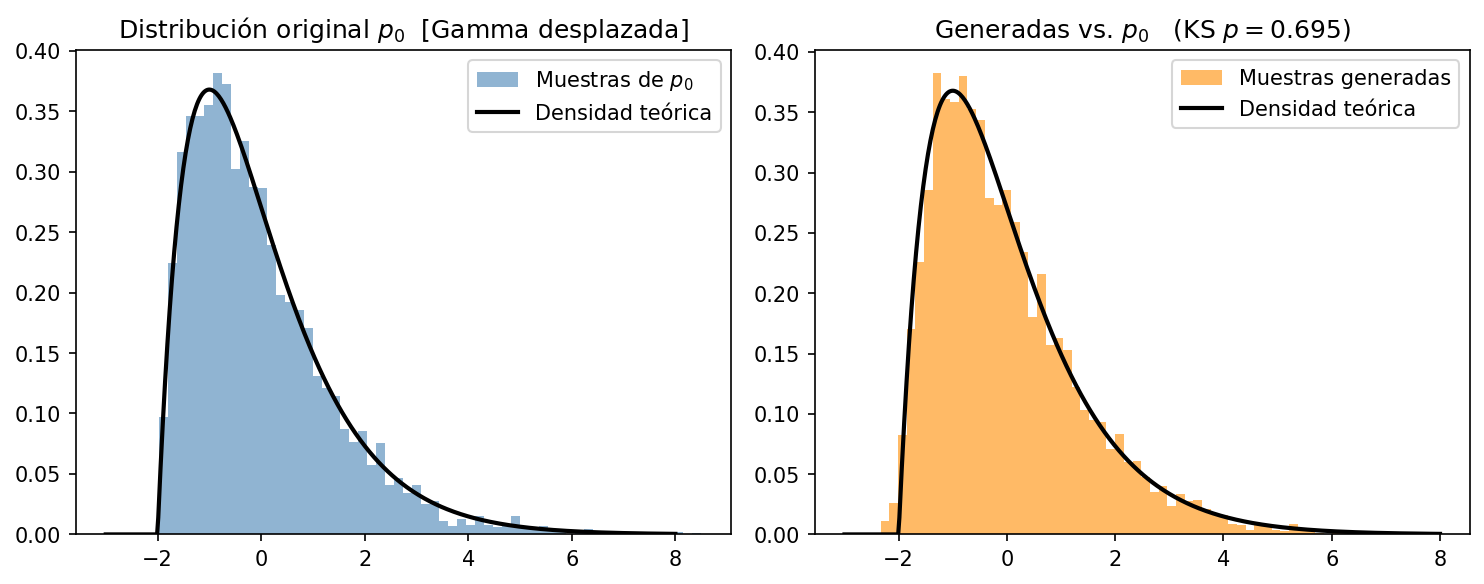
\includegraphics[width=\textwidth]{score_matching_demo.png}
  \caption{Izquierda: muestras reales de $p_0$ (Gamma desplazada) y su densidad teórica. Derecha: muestras generadas por el proceso inverso superpuestas a la misma densidad.}
  \label{fig:score-histograma}
\end{figure}

% ---- Bibliografía ----
\printbibliography[heading=bibintoc, title={Referencias}]

\end{document}
